% Last Update: $Id$
\marklabel{sec:opt-cpanel}
{
\section {OPT\_CPANEL}
}

\subsection{Einleitung}

Dieses Paket ermöglicht das Abfragen von 4 Tasten am seriellen Port des fli4l-Routers.
Bei Tastendruck werden Systemkommandos wie z.B. ``halt'' oder ``reboot'' aufgerufen. Die Tasten 
können frei belegt werden. Dabei sind 14 Variationen möglich (theoretisch sind 15 
möglich, allerdings macht bei der Nummer 15 die Hardware nicht mit). 

Die Power-LED leuchtet grün sobald die Schaltung einsatzbereit ist. Wird ein Befehl 
abgearbeitet, blinkt die LED. 
LED1 kann frei belegt werden (näheres erfahren Sie weiter unten).


\subsection{Tastenbelegung}

Die einzelnen Tastenbelegungen entsprechen der Stellenwertigkeit der Tasten.

\begin{itemize}
    \item Taste 1 = 1
    \item Taste 2 = 2
    \item Taste 3 = 4
    \item Taste 4 = 8
\end{itemize}

Sollen mehrere Tasten gleichzeitig betätigt werden, so addiert man die Stellenwertigkeit 
der einzelnen Tasten. Daraus erhählt man die Funktionsnummer für den Befehl.

Die auszuführenden Befehle werden in diese Zeilen eingetragen:
\var{OPT\_CPANEL\_FUNKTION1}='BEFEHL'
Dabei ist zu beachten, dass bei einigen Befehlen die komplette Pfadangabe zu dem Programm 
bzw. Skript angegeben werden muss.

Hierzu einige Beispiele:
\begin{verbatim}

fli4lctrl dial pppoe		Einwahl über DSL
fli4lctrl hangup pppoe		Trennen der DSL-Verbindung 
isdnctrl dial ippp0		Einwahl über ISDN
isdnctrl hangup ippp0		Trennen der ISDN-Verbindung
/sbin/reboot			Router neu starten
/sbin/halt			Router herunterfahren

\end{verbatim}

\subsection{Statusanzeige konfigurieren}

Es gibt vier Möglichkeiten die Status-LED zu belegen.

DSL: 

Es wird nur der DSL-Verbindungsstatus abgefragt und angezeigt.

ISDN: 

Es wird der ISDN-Verbindungsstatus abgefragt und angezeigt. Hierbei werden alle 
Circuits zusammengefasst. D.h. sobald ein Circuit online ist, leuchtet LED1.

DSLISDN:

Es wird der DSL- und der ISDN-Verbindungsstatus aller Circuits abgefragt 
und ausgegeben.

SCRIPT:

Hier können Sie ihre eigene Abfrage erstellen. Es ist dabei folgendes zu beachten:
\begin{itemize}
    \item Es müssen nur die Befehle eingetragen werden.
    \item \#!/bin/sh wird automatisch in das Script eingefügt.
    \item Damit die LED1 gesetzt wird, muss 'on' in die Datei /var/run/cpanel.status 
           geschrieben werden (natürlich ohne ' ').
    \item Um die LED wieder zu löschen, muss man 'off' in die Datei /var/run/cpanel.status 
           schreiben.
    \item Wird 'blink' in die Datei /var/run/cpanel.status geschrieben, blinkt LED1 bis 'off'
           oder 'on' gesetzt ist.
\end{itemize}

Beispiel:

Dies ist der Eintrag um den DSL-Status abzufragen:
\begin{verbatim}
echo off > /var/run/cpanel.status
fli4lctrl status | grep online >/dev/null && echo on > /var/run/cpanel.status
\end{verbatim}
Hinweis: 
Es sollte nur dann etwas eingetragen werden, wenn man sicher ist, was man
tut. Ein fehlerhafter Eintrag könnte zufolge haben das cpanel nicht startet
bzw. nicht richtig funktioniert.

\subsection{Fehlersuche}
\subsubsection{Hardware}

Sollte es nicht auf Anhieb funktionieren, überprüfen Sie zuerst ihre Schaltung.
Achten Sie dabei auf die richtige Pinbelegung am PC-Stecker. Sollte Ihr Router noch eine
25 polige Schnittstelle haben, gilt die Pinbelegung im Schaltplan nicht!
Wenn Sie die Schaltung überprüft haben und keinen Fehler gefunden haben, überprüfen Sie
das Kabel vom Mainboard zum Gehäuse. Da sich die Mainboardhersteller nicht auf einen
Standard einigen, gibt es verschiedene Adapterkabel. Überprüfen Sie gegebenfalls die
Pinbelegung des seriellen Steckers mit der Pinbelegung am Mainboardstecker
(siehe Mainboard-Handbuch).

\subsubsection{Software}

Zuerst sollten Sie überprüfen ob die cpanel-Software beim Booten startet. Dies kann man
daran erkennen das kurz vor dem Ende des Bootvorgangs eine Meldung ausgegeben wird. Sollte
dies nicht der Fall sein oder Sie haben sie übersehen, kann der Status auch mit 'ps ax'
auf der Konsole überprüft werden. Wenn cpanel nicht in der angezeigten Liste steht,
haben Sie vermutlich in der Datei config/cpanel.txt den Eintrag \var{OPT\_CPANEL}= auf 'no'
gestellt.
Eine weitere Fehlerquelle könnte die Grafikkarte sein. Wenn Sie keine Grafikkarte in
ihrem Router haben, wird der erste serielle Port (COM1) als Konsole verwedet. Dann muss
in der Datei config/cpanel.txt der Eintrag \var{CPANEL\_PORT}='/dev/ttyS0' auf '/dev/ttyS1'
umgestellt werden. Natürlich muss die Schaltung dann auch bei COM2 angesteckt sein.


\subsection{Allgemeines}

  \begin{figure}[htbp]
    \centering
    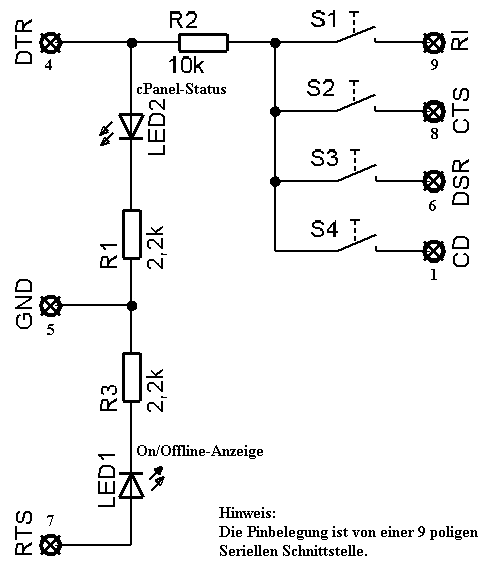
\includegraphics[width=485pt]{schematic}
    \caption{Der Schaltplan für die Schaltung}
    \label{fig:schaltplan}
  \end{figure}


\wichtig{Es wird keinerlei Haftung für evtl. Schäden übernommen!}

Probleme, Erfolgsberichte und Verbesserungsvorschläge bitte in die Newsgroup slpine.fli4l.opt posten.

Vielen Dank daß Sie diese Dokumentation gelesen haben. Viel 
Spaß mit cpanel!
